The evaluation is concerned with feasibility of the motion model and
simplicity for Web developers.


\subsection {Motion Synchronization}

We have used motion synchronization for a wide range of technical
demonstration since 2010. An early evaluation of the research prototype is
discussed in the paper titled \emph{The Media State Vector}~\cite{msv}. Though
the interpretations of the experiments are conservative, early findings
indicated that motion synchronization could provide frame rate levels of
accuracy (33 milliseconds). A few years later, a production ready service
called \emph{InMotion} was built by spin off company Motion
Corporation~\cite{mcorp}. With the introduction of
WebSockets~\cite{websocket}, results improved significantly. Synchronization
errors are in the order of a few milliseconds on all major browsers and most
operating systems (including Android). Typically we observe 0-1 millisecond
errors for desktop browsers, compared to a system clock synchronized by NTP.
The \emph{InMotion} service has also been running continuously for years,
supporting a wide range of technical demonstrations, at any time, at any
place, and across a wide range of devices. As such, the value of a production
grade online service is also confirmed.

Furthermore, the precision of motion synchronization degrades well with poor
network conditions. For instance, experiments with video synchronization in \emph{Enhanced Data rates for GSM Evolution (EDGE)}
connectivity has not been visibly worse, except for longer update
latency. In this instance, video data was fetched from local files.
Conferences are also notorious hotspots for bad connectivity. In these
circumstances, availability of media data consistently fails before
synchronization.


\subsection {Synchronization of HTML5 media elements}

Two technical reports~\cite{syncreport1,syncreport2} document the abilities
and limitations of HTML5 media elements with respect to media synchronization,
as well the quality of synchronization achieved by the \emph{MediaSync}
library. Synchronization errors of about 7 milliseconds is reported for both
audio and video, on desktops, laptops and high-end smartphones. This
corresponds to echoless audio playback. Smartphones and embedded devices such
a ChromeCast can be expected to provide frame accurate synchronization. 

These results have been consistently confirmed by day to day usage over
several years. The user experience of multi-device video synchronization is
also very good, to the point that errors are hardly visible, as demonstrated by
this video~\cite{carneval}. Echoless synchronization with the MediaSync
library may also produce various audio effects, like failing to hear one audio
source, until volume levels are changed and only the other audio source can be
heard. Since these effects are also achieved across browser types and
architectures, this is a strong indication that external timing is feasible
and already at a useful level.

Synchronization has also been maintained for hours and days at end, without
accumulated errors. Loading speeds are also acceptable. Even though the
MediaSync library requires about 3 seconds to reach echoless, the experience
is perceived as acceptable much before this. A variety of video demonstrations
have been published at the Multi-device Timing Community Group
Website~\cite{mtcg}.

\begin{figure}[h]
%\sidecaption
\centering
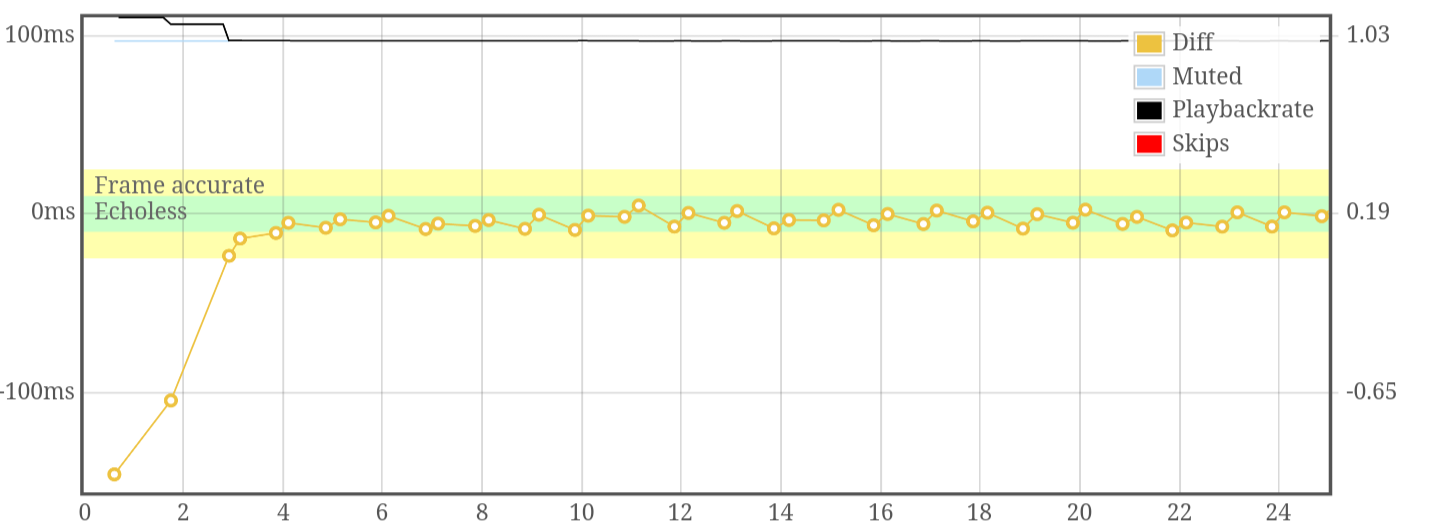
\includegraphics[scale=.23]{fig/android-video.png}
\caption{The figure illustrates an experiment with video (mp4) synchronization on
Android using Chrome browser. The plot shows currentTime compared to the ideal
playback position defined by motion. The X-axis denotes the timeline of the experiment (seconds).
The left Y-axis denotes difference \emph{Diff} (milliseconds) between currentTime and motion.
The green band (echoless) is +-10 millisecond and the yellow (frame accurate is) +-25 millisecond. 
This is achived using variable playbackRate. No skips were performed in this experiment. 
The right Y-axis denotes the value of playbackrate (seconds per second). The media element was muted until playbackrate stabilized.}
\label{fig:videosync}
\end{figure}

Though echoless synchronization is generally achievable, a lack of
standardization and common tests makes it impossible to provide any
guarantees. The experience might also be improved or become broken across
software updates. To be able to support echoless synchronization reliably
across browsers and devices, standards must include requirements for
synchronization, and testing-suites must be developed to ensure that those
requirements are met. Ideally though, media synchronization should be
implemented natively in media elements.


\subsection {Summary}

Interestingly, the results for motion synchronization and HTML5 media
synchronization are well aligned with current limitations of the Web platform.
For instance, the precision of timed operation in JavaScript is about 1
millisecond, and a 60Hz screen refresh rate corresponds to 16 milliseconds.
Furthermore, these results also match limitations in human sensitivity to
synchronization errors. 

Finally, programming synchronized media experiences in the motion model is
both easy and rewarding. In our experience, motions and sequencers are
effective thinking tools as well as programming tools. A globally synchronized
video experience essentially requires three code statements.

With this, we argue that the feasibility of the motion model is confirmed. It
is also clear that synchronization errors in online synchronization are
currently dominated by errors in synchronization in HTML5 media elements.
Future standardization efforts and optimizations would likely yield
significant improvements.